\documentclass[a4paper,landscape,8pt]{extarticle}

\usepackage[a4paper,margin=0.7cm]{geometry}

\usepackage{fancyhdr}
\pagestyle{fancy}
\fancyfoot[R]{\vspace{-35pt}\Huge\thepage}

\usepackage{multicol}
\setlength\columnsep{20pt}
\setlength{\columnseprule}{0.1pt} 

\setlength\parindent{0pt}

\usepackage[ngerman]{babel} % Silbentrennung
\usepackage[utf8]{inputenc} % Umlaute
\usepackage{microtype}

\usepackage{hyperref}

\usepackage{float}
\usepackage{graphicx}

\usepackage{comment}
\usepackage{amsmath}
\usepackage{amssymb}

\usepackage{cancel}

\usepackage{color}
\usepackage{xcolor}

\usepackage{color}

\usepackage{booktabs}

\newenvironment{rcases}
  {\left.\begin{aligned}}
  {\end{aligned}\right\rbrace}
  
\usepackage{enumitem}
\setlist{noitemsep,topsep=3pt,parsep=3pt,partopsep=3pt,leftmargin=18pt}
\renewcommand\labelitemi{{\boldmath$\cdot$}}
\newcommand{\listarrow}{
\smash{\scalebox{1.5}[1.75]{\rotatebox[origin=c]{180}{$\Lsh$}}}
}
\usepackage{xifthen}
\newcommand{\emptyarg}[1][]{\ifthenelse{\isempty{#1}}{}{\ #1}}

% % % % %
% Structural
% % % % %

\newcommand{\Def}[1][]{\colorbox{defcolor}{\color{titlecolor}{\textbf{D\emptyarg[#1]}}}\kern+0.3ex}

\newcommand{\Satz}[1][]{\colorbox{satzcolor}{\color{titlecolor}{\textbf{S\emptyarg[#1]}}}\kern+0.3ex}

\newcommand{\Theo}[1][]{\colorbox{lemcolor}{\color{titlecolor}{\textbf{T\emptyarg[#1]}}}\kern+0.3ex}

\newcommand{\Korollar}[1][]{\colorbox{lemcolor}{\color{titlecolor}{\textbf{K\emptyarg[#1]}}}\kern+0.3ex}

\newcommand{\Trick}[1][]{\colorbox{trkcolor}{\color{titlecolor}{\textbf{Trick:\emptyarg[#1]}}}\kern+0.3ex}

\newcommand{\Vorgehen}[1][]{\colorbox{trkcolor}{\color{titlecolor}{\textbf{Vorgehen:\emptyarg[#1]}}}\kern+0.3ex}

\newcommand{\Bsp}[1][]{\colorbox{bspcolor}{\color{titlecolor}{\textbf{B\emptyarg[#1]}}}\kern+0.3ex}

% % % % %
% In Text
% % % % %

\newcommand{\Bem}{\textbf{Bem: }}
\newcommand{\Beweis}{\textbf{Beweis: }}
\newcommand{\Achtung}{\textbf{Achtung: }}
\newcommand{\Wichtig}{\textbf{Wichtig: }}

% % % % %
% Colors
% % % % %

\definecolor{defcolor}{rgb}{0.5, 1, 0.5}
\definecolor{satzcolor}{rgb}{0.5, 0.95, 1}
\definecolor{lemcolor}{rgb}{1, 0.75, 0.75}
%\definecolor{trkcolor}{rgb}{1, 0.7, 0}
\definecolor{trkcolor}{rgb}{0.7, 0.95, 1}
\definecolor{bspcolor}{rgb}{1, 0.95, 0.43}
\definecolor{titlecolor}{rgb}{0,0,0}

% % % % %
% Math
% % % % %

\DeclareMathOperator{\arcsinh}{arcsinh}
\DeclareMathOperator{\arccosh}{arccosh}
\DeclareMathOperator{\arctanh}{arctanh}
\DeclareMathOperator{\arc}{arc}

\renewcommand\div{\operatorname{div}}
\DeclareMathOperator{\rot}{rot}
\newcommand{\laplace}{\Delta}

\DeclareMathOperator{\cis}{cis}

\DeclareMathOperator{\grad}{grad}
\DeclareMathOperator{\Hess}{Hess}

\newcommand{\N}{\mathbb{N}}
\newcommand{\Z}{\mathbb{Z}}
\newcommand{\Q}{\mathbb{Q}}
\newcommand{\R}{\mathbb{R}}
\newcommand{\C}{\mathbb{C}}


\renewcommand\Re{\operatorname{Re}}
\renewcommand\Im{\operatorname{Im}}

\newcommand{\abs}[1]{\left\lvert #1 \right\rvert}
\newcommand{\norm}[1]{\left\lVert #1 \right\rVert}
\newcommand{\scprod}[1]{\left\langle #1 \right\rangle}
\newcommand{\ceil}[1]{\left\lceil #1 \right\rceil}
\newcommand{\floor}[1]{\left\lfloor #1 \right\rfloor}

\newcommand{\diag}{\operatorname{diag}}

\newcommand{\hl}[1]{\colorbox{black!7}{$#1$}}

\newcommand{\notimplies}{\;\not\!\!\!\implies}

% % % % %
% Layout
% % % % %

\newcommand{\setsep}{\ \vert \ }

\newcommand{\todo}{\textcolor{red}{TODO }}

\newcommand{\sep}{\vspace{5pt}\noindent\hrule\vspace{5pt}}


\newcommand{\veryshortarrow}[1][3pt]{\mathrel{%
   \hbox{\rule[\dimexpr\fontdimen22\textfont2-.2pt\relax]{#1}{.4pt}}%
   \mkern-4mu\hbox{\usefont{U}{lasy}{m}{n}\symbol{41}}}}
% TODO remove command
\renewcommand*{\newpage}{ \ }
%\renewcommand*{\part}{\ }
% package to define custom environments
\usepackage{environ}
% boolean variable to show contents
\newif\ifshowwarmup
%\showwarmuptrue % set it to true
\showwarmupfalse % set it to false
% definition of custom environment
\NewEnviron{warmup}{\ifshowwarmup \BODY \fi}
% shorthand for custom environment
%\def\WU#1\UW{\begin{warmup}#1\end{warmup}}
% Ultra shortening of Document
%
% http://www.terminally-incoherent.com/blog/
%2007/09/19/latex-squeezing-the-vertical-white-space/
%\setlength{\parskip}{0pt}
%\setlength{\parsep}{0pt}
%\setlength{\headsep}{0pt}
\setlength{\topskip}{0pt}
%\setlength{\topmargin}{0pt}
%\setlength{\topsep}{0pt}
%\setlength{\partopsep}{0pt}
%\linespread{0.7}
\usepackage[compact]{titlesec}
\titlespacing{\section}{0pt}{*0}{*0}
\titlespacing{\subsection}{0pt}{*0}{*0}
\titlespacing{\subsubsection}{0pt}{*0}{*0}
%\usepackage{savetrees} %(alternative)
\pagenumbering{gobble}
% Use custom numbering
%\setcounter{secnumdepth}{0}
\usepackage{centernot}
\begin{document}
\setlength{\belowdisplayskip}{4pt} \setlength{\belowdisplayshortskip}{4pt}
\setlength{\abovedisplayskip}{4pt} \setlength{\abovedisplayshortskip}{4pt}
% allow page break in align* environment
\allowdisplaybreaks
\begin{multicols*}{4} % change to 3 if you want only 3 columns
\raggedcolumns
\graphicspath{ {./img/} }
\section*{Grundlagen}
\Def[1.1Sigma-Algebra ]
\begin{itemize}
    \item \(\omega \in \mathcal{F}\)
    \item  \(A \in \mathcal{F} \implies A^c \in \mathcal{F}\)
    \item \(A_1, A_2, \dots \in \mathcal{F} \implies \bigcup_{i=1}^{\infty} A_i \in \mathcal{F} \)
\end{itemize}
\Def[1.2 Wahrscheinlichkeitsmass ]
\begin{itemize}
    \item \( \mathcal{P}[\omega] = 1\)
    \item \(\sigma-\text{Additivität} \ \mathcal{P}[A] = \sum_{i=1}^{\infty} \mathcal{P}[A_i]\) \newline if \( A = \bigcup_{i=1}^{\infty} A_i \) (disjunkte Vereinigung)
\end{itemize}
\Def[1.3 Wahrscheinlichkeitsraum ] \\
Sei \( \omega \) ein Grundraum, \(\mathcal{F}\) eine \(\sigma\) -Algebra und \(\mathcal{P}\) ein Wahrscheinlichkeitsmass. Wir nennen das Tripel\( (\omega, \mathcal{F}, \mathcal{P})\)  Wahrscheinlichkeitsraum.
\Def[1.5 Laplace Modell] \\
\begin{itemize}
    \item \(\mathcal{F} = \mathcal{P}(\omega)\)
    \item \(\mathbb{P} : \rightarrow \left[0,1\right]\) ist definiert durch \[ \forall A \in \mathcal{F} \ \mathbb{P}[A] = \frac{\abs{A}}{\abs{\omega}}\]
\end{itemize}
\Satz[1.6]
Für eine Sigma-Algebra \(\mathcal{F} \ \text{auf} \ \omega\) gilt:
\begin{itemize}
    \item \(\emptyset \in \mathcal{F}\)
    \item \(A_1, A_2, \dots \in \mathcal{F} \implies \bigcap_{i=1}^{\infty} A_i \in \mathcal{F}\)
    \item \(A,B \in \mathcal{F} \implies A \cup B \in \mathcal{F}\)
    \item \(A,B \in \mathcal{F} \implies A \cap B \in \mathcal{F}\)
\end{itemize}
\Satz[1.7]
\begin{itemize}
    \item \( \mathbb{P}[\emptyset] = 0\)
    \item \(A_1, \dots A_k\) paarweise disjunkte Ereignisse, \[\mathbb{P}[A_1 \cup \dots \cup A_k] = \mathbb{P}[A_1] + \dots \mathbb{P}[A_k]\]
    \item \( \mathbb{P}[A^c] = 1 - \mathbb{P}[A]\)
    \item \(\mathbb{P}[A \cup B ] = \mathbb{P}[A] - \mathbb{P}[B] - \mathbb{P}[A \cap B]\)
\end{itemize}
\Satz[1.8] Seien \(A,B \in \mathcal{F}\) dann gilt \[ A \subset B \implies \mathbb{P}[A] \leq \mathbb{P}[B]\]
\Satz[1.9] Sei \( A_1, A_2, \dots \) eine Folge von nicht notwendigerweise disjunkten Ereignissen, dann gilt: \[ \mathbb{P}[\bigcup_{i=1}^{\infty} A_i \leq \sum_{i=1}^{\infty} \mathbb{P}[A_i]]\]
\Def[1.13 Bedingte Wahrscheinlichkeit] \newline
Sei \((\omega, \mathcal{F}, \mathbb{P})\) ein Wahrscheinlichkeitsraum. Seien A, B zwei Ereignisse mit \( \mathbb{P}[B] > 0\) \[\mathbb{P}[A|B] = \frac{\mathbb{P}\left[A \cap B\right]}{\mathbb{P}\left[B\right]}\]
\Satz[1.16 Gesetz der totalen Wahrscheinlichkeit] \newline
Sei  \( B_1, \dots , B_n\) eine Partition des Grundraumes \( \omega \), so dass \( \mathbb{P}[B_i] > 0 \) für jedes \( 1 \leq i \leq n\) gilt. Dann gilt: \[\forall A \in  \mathcal{F} \ \mathbb{P}[A] = \sum_{i=1}^{n} \mathbb{P} \left[A | B_i \right] \mathbb{P}[B_i]\]
\Satz[1.17 Satz von Bayes] \newline
Sei \( B_1 \dots B_n \in \mathcal{F }\) eine Partition von \( \omega\) sodass, \( \mathbb{P}[B_i] > 0 \) für jedes i gilt. Für jedes Ereignis A mit \( \mathbb{P}[A] > 0 \) gilt  \[ \forall i = 1, \dots n \ \mathbb{P}\left[ B_i | A \right] = \frac{\mathbb{P}[A | B_i] \mathbb{P}[B_i]}{\sum_{j=1}^{n} \mathbb{P}[A | B_j] \mathbb{P}[B_j] }\]
\Def[1.18 Unabhängigkeit] \newline
Sei \( (\omega, \mathcal{F}, \mathbb{P})\) ein Wahrscheinlichkeitsraum. Zwei Ereignisse A und B heissen unabhängig falls \[ \mathbb{P} \left[A \cap B \right] = \mathbb{P}\left[A\right] \mathbb{P} \left[B\right]\]
\Satz[1.20] \newline
Seien A,B \( \in \mathcal{F}\) zwei Ereignisse mit \( \mathbb{P}[A], \mathbb{P}[B] > 0 \). Dann sind folgende Aussagen äquivalent:
\begin{enumerate}
    \item \( \mathbb{P}[A \cap B] = \mathbb{P}[A] \mathbb{P}[B]\)
    \item \( \mathbb{P}[A | B] = \mathbb{P}[A]\)
    \item \( \mathbb{P}[B | A] = \mathbb{P}[B]\)
\end{enumerate}
\Def[1.21]  \newline
Sei I eine beliebige Indexmenge. Eine Familie von Ereignissen \( (A_i)_{i \in I}\) heisst unabhängig falls \[ \forall J \subset I \text{endlich} \quad \mathbb{P}[\bigcap_{j \in J}A_j] = \prod_{j \in J} \mathbb{P}[A_j]\]
\Bem \newline
Drei Ereignisse A,B und C sind unabhängig falls alle 4 folgenden Gleichungen erfüllt sind
\begin{enumerate}
    \item \( \mathbb{P}[A \cap B ] = \mathbb{P}[A] \mathbb{P}[B]\)
    \item \( \mathbb{P}[A \cap C ] = \mathbb{P}[A] \mathbb{P}[C]\)
    \item \( \mathbb{P}[B \cap C ] = \mathbb{P}[B] \mathbb{P}[C]\)
    \item \( \mathbb{P}[A \cap B \cap C  ] = \mathbb{P}[A] \mathbb{P}[B] \mathbb{P}[C]\)
\end{enumerate}
\sep
\section{Zufallsvariablen und Verteilungsfunktionen}
\subsection{Abstrakte Definition }
\Def[2.1 Zufallsvariable] \newline
Sei \( (\omega, \mathcal{F}, \mathbb{P})\) ein Wahrscheinlichkeitsraum. Eine Zufallsvariable ist eine Abbildung \( X : \omega \rightarrow \mathbb{R} \) so dass, für alle \( a \in \mathbb{R}\) gilt \[ \{ w \in \omega : X(w) \leq a \} \in \mathcal{F}\]
\Bem  \newline
Für Ereignisse im Bezug auf Z:V
\begin{itemize}
    \item \( \{X \leq a \} = \{ w \in \omega : X(w) \leq a\}\)
    \item \( \{ a < X \leq b \} = \{ w \in \omega : a < X(w) < b\}\)
    \item \( \{ X \in \mathbb{Z}\} = \{ w \in \omega : X(w) \in \mathbb{Z}\}\)
\end{itemize}
\[ \mathbb{P}[X \leq a] = \mathbb{P}[\{X \leq a\}] = \mathbb{P}[\{w \in \omega : X(w) \leq a\}]\]
\subsection{Verteilungsfunktion}
\Def[2.2 Verteilungsfunktion] \newline
Sei X eine Zufallsvariable auf einem W-Raum \( (\omega, \mathcal{F}, \mathbb{P})\). Die Verteilungsfunktion von X ist eine Funtkion \(F_X : \mathbb{R} \rightarrow [0,1]\), definiert durch \[ \forall a \in \mathbb{R} \ F_X(a) = \mathbb{P}[X \leq a]\]
\Satz[2.3 Einfache Identität] \newline
Seien \(a < b\) zwei reelle Zahlen. Dann gilt \[ \mathbb{P}[a < X \leq b ] = F(b) - F(a)\]
\Theo[2.4 Eigenschaften der Verteilungsfunktion] \newline
Sei X eine Z.V aif einem Wahrscheinlichkeitsraum. Die Verteilungsfunktion \( F = F_X : \R \rightarrow [0,1]\) von X erfüllt folgende Eigenschaften
\begin{itemize}
    \item F ist monoton wachsend
    \item F ist rechtsstetig
    \item \( \lim_{a \rightarrow -\infty} F(a) = 0 \) und \( \lim_{a \rightarrow \infty} F(a) = 1\)
\end{itemize}
\subsection{Unabhängigkeit von Zufallsvariablen}
\Def[2.5] \newline
Seien \( X_1 \dots X_n \) Zufallsvariablen auf einem W-Raum. Dann heissen \(X_1, \dots X_n \) unabhängig falls \[ \forall x_1, x_2 \dots x_n \in \R \] \[\mathbb{P}[X_1 \leq x_1 \dots X_n \leq x_n ] = \mathbb{P}[X_1 \leq x_1] \dots \mathbb{P}[X_n \leq x_n]\]
\Satz[2.7 Gruppieren von Zufallsvariablen] \newline
Seien \(X_1 \dots X_n\) n unabhängige Zufallsvariablen. Seien \( 1 \leq i_1 < i_2 < \dots < i_k \leq n \) Indizes und \(\phi_1 \dots \phi_k\) Abbildungen. Dann sind  \[ Y_1 = \phi_1(X_1 \dots X_{i_1}), Y_2 = \phi_2(X_{i_{1}+1}, \dots X_{i_2}), \dots \] \[Y_k = \phi_k(X_{i_{k-1}+1} \dots X_{i_k})\] unabhängig \newline
\newline \newline
\Def[2.8] \newline
Eine Folge von Zufallsvariablen \(X_1, X_2, \dots \) heisst
\begin{itemize}
    \item unabhängig falls \(X_1, \dots X_n \) unabhängig sind, für alle \(n \in  \N\)
    \item unabhängig und identisch verteilt(uiv) falls sie unabhängig ist und die Zufallsvariablen dieselbe Verteilungsfunktion haben d.h \[ \forall i, j \ F_{X_i} = F_{X_j}\]
\end{itemize}
\subsection{Konstruktion von Zufallsvariablen}
\Def[2.9] \newline
Sei \(p \in [0,1]\). Eine Zufallsvariable X heisst Bernoulli ZUfallsvariable mit Parameter p falls \[\mathbb{P}[X=0] = 1 - p \ \text{und} \ \mathbb{P}[X=1] = p\]
Dabei schreiben wir \( X \sim Ber(p)\)
\Theo[2.10 Existenzsatz von Kolmogorov] \newline
Es existiert ein W-Raum \( (\Omega, \mathcal{F}, \mathbb{P}) \) und eine nicht endliche uiv Folge von Bernoulli Zufallsvariablen \(X_1, X_2, \dots \) auf \( (\Omega, \mathcal{F}, \mathbb{P}) \) mit Paramter \(\frac{1}{2}\)
\Def[2.11] \newline
Eine Zufallsvariable U heisst gleichverteilt auf \([0,1]\) falls ihre Verteilungsfunktion gegeben ist durch\[F_U(x) = \left.
    \begin{cases}
    0 & x < 0 \\
    x & 0 \leq x \leq 1 \\
    1 &  x > 1
\end{cases}
\right.\]
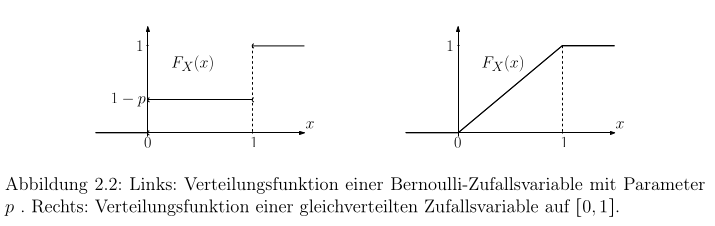
\includegraphics[scale=0.3]{abb2.2.png}
\Def[2.13 Pseudoinverse] \newline
Die Pseudoinverse von F ist eine Abbildung \(F^{-1} : (0,1) \rightarrow \R \) definiert durch \[ \forall \alpha \in (0,1) \ F^{-1} = \inf{x \in \R : F(x) \geq \alpha}\]
Nach Definition des Infimums und unter Verwendung der rechten Stetigkeit von F ergibt sich für jedes \(x \in \R \) und \( \alpha \in (0,1)\)
\[ (F^{-1}(\alpha) \leq x ) \Leftrightarrow (\alpha \leq F(x))\]
\Theo[2.14 Inversionsmethode] \newline
Sei \(F: \rightarrow [0,1]\) eine Abbildung, welche Eigenschaften 1-3 erfüllt. Sei U eine Gleichverteilte Zufallsvariable. Dann besitzt die Zufallsvariable
\[X = F^{-1}(U)\]
gerade die Verteilungsfunktion \(F_X = F\)

\sep
\section{Diskrete und stetige Variablen}
\subsection{Unstetigkeit/Stetigkeit der Verteilungsfunktion F}
\Satz[3.1 Wahrscheinlichkeit eines Punktes] \newline
Sei \( X : \omega \rightarrow \R \) eine Zufallsvariable mit Verteilungsfunktion F. Für jdedes a in \(\R\) gilt \[ \mathbb{P}[X = a] = F(a) - F(-a)\]
\subsection{Fast sichere Ereignisse}
\Def[3.2] \newline
Sei \( A \in \mathcal{F} \) ein Ereignis. Wir sagen A tritt fast sicher ein falls \[ \mathbb{P}[A] = 1\]
\subsection{Diskrete Zufallsvariablen}
\Def[3.4 Diskrete Zufallsvariable] \newline
Eine Zufallsvariable \( X : \omega \rightarrow \R \) hiest diskret falls eine endliche oder abzählbare Menge \( W \subset \R\) existiert, sodass \[ \mathbb{P}[X \in W ] = 1\]
\Bem[3.5] Wenn der Grundraum \( \omega\) endlich oder abzähbar ist, dann ist jede Zufallsvariable \( X : \omega \rightarrow \R\) diskret. \newline
\Def[3.6 Verteilung von X] \newline
Sei X eine diskrete Zufallsvariable mit Werten in einer endlichen oder abzähbaren Menge \( W \subset \R\). Die Zahlenfolge \((p(x))_{x \in W}\) definiert durch \[ \forall x \in W \ p(x) := \mathbb{P}[X = x]\] heisst Verteilung von X \newline
\Satz[3.7] Die Verteilung \((p(x))_{x \in W}\) einer diskreten Zufallsvariable erfüllt \[ \sum_{x \in W} p(x) = 1\]
\Satz[3.9] Sei X eine diskrete Zufallsvariable, dessen WErte in einer endlichen oder abzähbaren Menge W liegen, und deren Verteilung p ist. Dann ist die Verteilungsfunktion von X gegeben durch \[ \forall X \in \R \ F_X(x) = \sum_{y \leq x_{y \in W}}p(y)\]
\subsection{Beispiele diskreter Zufallsvariablen}
\Def[3.10 Bernoulli Verteilung] \newline
Es sei \( 0 \leq p \leq 1\). Eine Zufallsvariable X heisst Bernoulli Zufallsvariable mit Parameter p, wenn sie Werte in W \( = \{0,1\}\) annimt und folgendes gilt \[ \mathbb{P}[X=0] = 1-p \quad \text{und} \ \mathbb{P}[X=1] = p\]
\Def[3.11 Binomialverteilung] \newline
Sei \( 0 \leq p \leq 1\), sein \( n \in \N\). Eine Zufallsvariable X heisst binomiale Zufallsvariable mit Paramtern n und p, wenn sie werte in \( W = \{ 0, \dots , n\}\) annimt und folgendes gilt \[\forall k \in \{0, \dots , n\} \ \mathbb{P}[X=k] = \binom{n}{k} p^k(1-p)^{n-k}\]
\Satz[3.13 Sum von unab. Bern. und Binom. Z.V] \newline
Sei \( 0 \leq p \leq 1\), sein \( n \in \N\). Seien \( X_1, \dots, X_n\) unabhängige Bernoulli Z.V mit Parameter p. Dann ist \[ S_n := X_1 + \dots + X_n\] eine binomialverteilte Z.V mit paramtern n und p.
\Bem[3.14] \newline
Bin(1,p) ist gerade Ber(p) verteilt. Falls \(X \sim Bin(m,p), Y \sim Bin(n,p) \) und X,Y unabhängig, dann ist \(X + Y \sim Bin(m+n, p)\)  verteilt.
\Def[3.15 Geometrische Verteilung] \newline
Es sei \( 0 < p \leq 1\). Eine Zufallsvariable X heisst geometrische Zufallsvariable mit Parameter p, falls sie Werte in W = \( \N \setminus \{0\}\) annimt und folgendes gilt \[\forall k \in \N \setminus \{0\} \ \mathbb{P}[X=k] = (1-p)^{k-1} \cdot p\]
\Bem[3.16] \newline
Für p=1 und k = 1 erscheint in der obigen Gleichung \(0^0 = 1\) , es gilt \( \mathbb{P}[X=1] = p\) \newline
\Satz[3.18] \newline
Sei \(X_1, X_2, \dots \) eine Folge von unendlich vielen unabhängigen Bernoulli Z.V mit Parameter p. Dann ist \[ T:= \min\{n \geq 1 : X_n = 1\}\] eine geometrisch verteilte Zufallsvariable mit Paramter p. \newline
\Bem[3.18A] \newline
Sei T eine geometrische Verteilung mit Parameter p. Dann ist \( T > n\), wenn die ersten n Bernoulli-Experimente fehlschlagen. Daher gilt \[ \mathbb{P}[T > n] = (1-p)^n\]
\Satz[3.20 Gedächnislosigkeit der Geo. Vert.] \newline
Sei \( T \sim Geom(p)\) für \( 0 < p < 1\). Dann gilt \[ \forall n \geq 0 \quad \forall k \geq 1 \quad \mathbb{P}[T \geq n + k | T > n] = P[T \geq k]\]
\Def[3.21] \newline
Sei \( \lambda > 0\) eine positive reelle Zahl. Eine Zufallsvariable X heisst Poisson-Zufallsvariable mit Paramter \( \lambda\), wenn sie Werte in \( W = \N \) annimt und folgendes gilt \[ \forall k \in \N \ \mathbb{P}[X = k] = \frac{\lambda^k}{k!}\exp^{-\lambda}\]
\Satz[3.23 Poisson-Approx. der Binom. verteil.] \newline
Sei \( \lambda > 0\). Für jedes \( n \geq 1 \) seien \( X_n \sim Bin(n, \frac{\lambda}{n})\)  Zufallsvariablen. Dann gilt \[ \forall k \in \N \ \lim_{n \rightarrow \infty } \mathbb{P}[X_n = k] = \mathbb{P}[N =k]\]
\subsection{Stetige Verteilungen}
\Def[3.25 Stetig verteilte Zufallsvariablen] \newline
Eine Zufallsvariable \( X: \omega \rightarrow \R \) heisst stetig, wenn ihre Verteilungsfunktion \(F_X \) wie folgt geschrieben werden kann \[F_X(a) = \int_{-\infty}^{a} f(x)dx \ \text{für alle a in} \ \R\] wobei \(f: \R \rightarrow \R_+\) eine nicht-negative Funktion ist. Wir nennen dann f Dichte von X. Weiter gilt für f \[1 = \int_{-\infty}^{\infty} f(x) dx\] \newline
\Bem[3.25A] \newline
\(f(x)dx \) ist die Wahrscheinlichkeit, dass X Werte in \( [x, x+ dx]\) annimmt. Die Stetigkeit von \(F_X \)folgt dabei aus der Definition (3.25). Ausserdem folgt aus Satz 3.1, dass \[ \forall x \in \R  \ \mathbb{P}[X = x] = 0\]Die Wahrscheinlichkeit für das Auftreten jedes einzelnen Werts der Zufallsvariablen beträgt exakt Null\newline
\Bem[3.25B] \newline
Von f zu \( F_X\) : Sei X eine stetige Z.V und f die Dichte. \(F_X\) können wir mit \[F_X(x) = \int_{-\infty}^x f(y)dy\] Es liegt nahe, dass wir die Dichte mittels Ableiten herausfinden \newline
\Theo[3.26] \newline
Sei X eine Zufallsvariable. Die Verteilungsfunktion \(F_X\) sei stetig und Stückweise \( C^1\), d.h es gibt \(x_0 = -\infty < x_1 < \dots < x_{n-1} < x_n = + \infty\), sodass \(F_X\) auf jedem Intervall \( (x_i, x_{i+1})\) Element von \(C^1\) ist. Dann ist X eine stetige Zufallsvariable und die Dichte f kann konstruiert werden, indem man folgendes festlegt \[ \forall x \in (x_i, x_{i+1}) \ f(x) = F'_X(x)\]
\subsection{Beispiele stetiger Zufallsvariablen}
\Def[3.27 Gleichverteilung auf [a,b]] \newline
Eine stetige Zufallsvariable X heisst gleichverteilt auf \([a,b]\) falls ihre Dichte gegeben ist durch \[ f_{a,b}(x) = \begin{cases}
    \frac{1}{b-a} & x \in [a,b] \\
    0 & x \notin [a,b]
\end{cases}\]
Wir schreiben \(X \sim \mathcal{U}([a,b])\) \newline
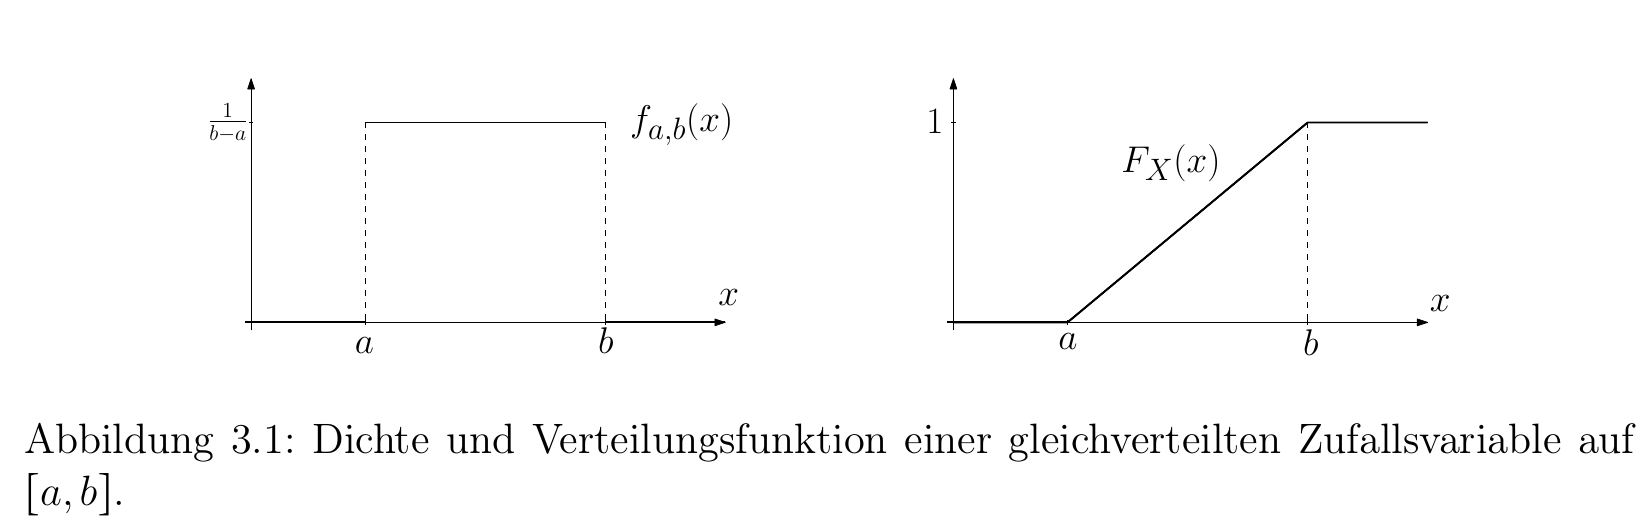
\includegraphics[scale=0.1]{Gleichverteilt.png}
\Bem[3.27A]
\begin{itemize}
    \item Die Wahrscheinlichkeit in einem Interval \( [c, c + \ell] \subset [a,b]\) zu fallen ist lediglich abhängig von dessen Länge \( \ell\) \[\mathbb{P}[X \in [c, c + \ell ]] = \frac{\ell}{b-a}\]
    \item Die Verteilungsfunktion X ist gegeben durch \[ F_X(x) = \begin{cases}
        0 & x < a \\
        \frac{x-a}{b-a} & a \leq x \leq b \\
        1 & x > b
    \end{cases}\]
\end{itemize}
\Def[3.28 Exponentialverteilung mit \(\lambda > 0\) ] \newline
Eine stetige Zufallsvariable T heisst exponentialverteilt mit Parameter \( \lambda > 0\) falls ihre Dichte gegeben ist durch
\[ f_\lambda(x) = \begin{cases}
    \lambda \exp ^{-\lambda x } & x \geq 0 \\
    0 & x < 0
\end{cases}\]
\Bem[3.28A]
Die Grafik zeigt die Dichte und Verteilungsfunktion einer exponentialverteilten Zufallsvariable mit Parameter \( \lambda\)
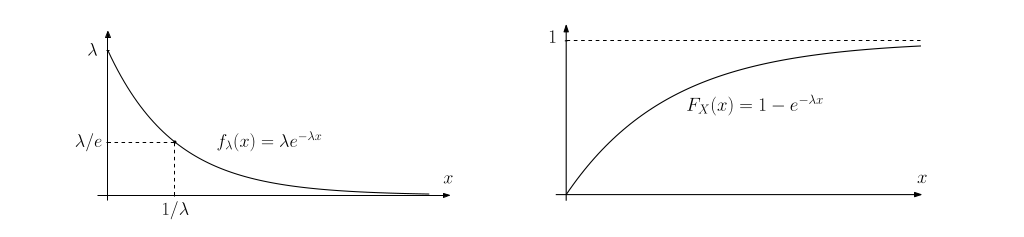
\includegraphics[scale=0.2]{exp_Dichte_Verteilung.png} \\ 
T modelliert häufig die Lebensdauer oder Wartezeit eines allgemeinen Ergebnisses. \\
Eigenschaften: \begin{itemize}
    \item Die Wahrscheinlichkeit des Wartens ist exponentiell klein: \[ \forall t \geq 0 \ \mathbb{P}[T > t] = \exp^{-\lambda t }\]
    \item T besitzt die Eigenschaft der Gedächnislosigkeit \[ \forall t,s > 0 \ \mathbb{P}[T > t + s | T > t] = [T > s]\]
\end{itemize}

\Def[3.29] \newline
Eine stetige Zufallsvariable X heisst normal verteilt mit Parametern m und \( \sigma^2 > 0\) falls ihre Dichte gegeben ist durch \[ f_{m,\sigma}(x) = \frac{1}{\sqrt{2 \pi \sigma^2}}\exp^{-\frac{(x-m)^2}{2 \sigma^2}}\]
Wir schreiben \( X \sim \mathcal{N}(m, \sigma^2)\) \newline
\Bem[3.29A] \newline
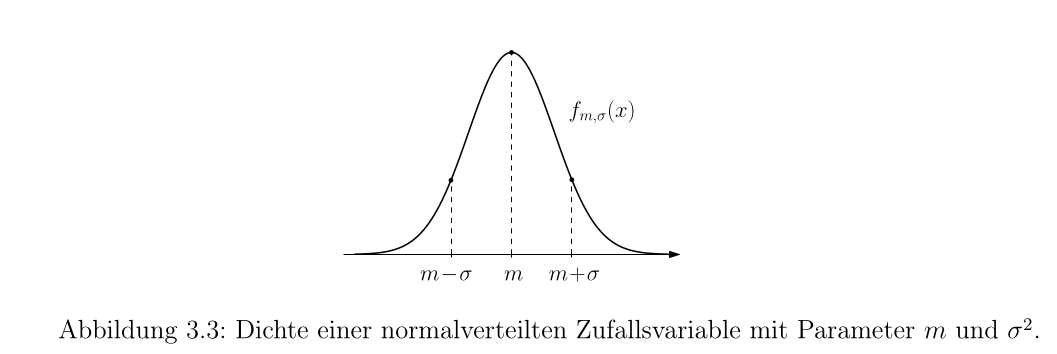
\includegraphics[scale=0.175]{Dichte_Normalverteilung.png} \\
Zum Beispiel bei einer physikalischen Messung kann der parameter \( \sigma\) die Schwankung von X darstellen und generell zeigt ein kleines \(\sigma\) eine genaue Messung an und ein grosses \(\sigma\) eine ungenaue.
Eigenschaften : \begin{itemize}
    \item Seien \(X_1, \dots X_n\) unabhängige normalverteilte Zufallsvariablen mit Parametern \((m_1, \sigma_1^2), \dots , (m_n, \sigma_n^2)\) dann ist \[ Z = m_0 + \lambda_1 X_1 + \dots + \lambda_n X_n \] eine normalverteilte Zufallsvariable mit Parametern \(m = m_0 + \lambda_1 m_1 + \dots + \lambda_n m_n\) und \(\sigma^2 = \lambda_1^2 \sigma_1^2 + \dots + \lambda_n^2 \sigma_n^2\)
    \item Wir sprechen im Fall von  \( X \sim \mathcal{N}(0,1)\), gerade von einer standardnormalverteilten Zufallsvariable. Man merke sich dann folgende Beziehung \[ Z = m + \lambda \cdot X\], wobei X eine normalverteilte Zufallsvariable mit Parametern m und \(\sigma^2\) ist.
    \item Falls X normalverteilt mit Parametern m und \( \sigma^2 \) ist, dann liegt die "meiste " Wahrscheinlichkeitsmasse der Z.V im Intervall \( [m - 3\sigma, m + 3\sigma ]\). Es gilt gerade \[ \mathbb{P}[\abs{X - m} \geq 3 \sigma ] \leq 0.0027\]
\end{itemize}


\sep
\section{Der Erwartungswert}
\subsection{Der allgemeine Erwartungswert}
\Def[4.1] \newline
Sei \( X : \omega \rightarrow \R_+ \) eine Zufallsvariable mit nicht-negativen Werten. Dann heisst \[ \mathbb{E}[X] = \int_0^\infty (1-F_X(x)) dx\] der Erwartungswert von X. \newline
\Bem[4.2] \newline
Der Erwartungswert kann sowohl endliche als auch nicht endliche Werte annehmen. Für allgemeinen ZV. definieren wir den Erwartungswert durch Zerlegen in einen positiven und negativen Teil. Die Beiden Zufallsvariablen sind wie folgt definiert : \[X_+(\omega) = \begin{cases}
    X(\omega) & \text{falls} X(\omega) \geq 0 \\
    0 & \text{falls} X(\omega) < 0
\end{cases}\]
und \[X_-(\omega) = \begin{cases}
    -X(\omega) & \text{falls} X(\omega) \leq 0 \\
    0 & \text{falls} X(\omega) > 0
\end{cases}\]
\(X_+ \) und \(X_-\) sind nicht negative Zufallsvariablen. Zudem gilt \(X = X_+ - X_-\) als auch \( \abs{X} = X_+ + X_-\)
\Satz[4.3] \newline
Sei X eine nicht-negative Zufallsvariable. Dann gilt \[ \mathbb{E}[X] \geq 0\]
\Def[4.4] Sei X eine Zufallsvariable. Falls \(\mathbb{E}[\abs{X}] < \infty \), dann heisst \[ \mathbb{E}[X] = \mathbb{E}[X_+] - \mathbb{E}[X_-]\] Erwartungswert von X. \newline
\Bsp[4.5] \newline Sei X eine Bernoulli Z.V mit Parameter p \[\mathbb{E}[X] = p\] Sei X Poisson-verteilt mit Parameter \( \lambda > 0\) \[\mathbb{E}[X] = \lambda\] Sei \(A \in \mathcal{F}\) ein Ereignis. Sei \( \mathbbm{1}_A \) die Indikatorfunktion auf A, \[ \forall \omega \in \Omega \ \mathbbm{1}_A(\omega) = \begin{cases}
    0 & \text{falls} \omega \notin A \\
    1 & \text{falls} \omega \in A
\end{cases}\]
Dann ist \(\mathbbm{1}_A\) eine Zufallsvariable. Per Definition gilt \[\mathbb{P}[X = 0] = 1 - \mathbb{P}[A] \ \text{und} \ \mathbb{P}[X=1] = \mathbb{P}[A]\]
Somit ist \(\mathbbm{1}_A\) eine Bernoulli Z.V mit Paramter \( \mathbb{P}[A] \ \implies \mathbb{E}[\mathbbm{1}_A] = \mathbb{P}[A]\) \newline
\subsection{Erwartungswert einer diskreten Zufallsvariable}
\Satz[4.6] Sei \( X: \omega \rightarrow \R \) eine diskrete Zufallsvariable dessen Werte in W (endlich oder abzähbar ) fast sicher liegen.Dann gilt \[ \mathbb{E}[X] = \sum_{x \in W} x \cdot \mathbb{P}[X = x]\]
\Satz[4.7] Sei \( X: \omega \rightarrow \R \) eine diskrete Zufallsvariable mit Werten in W (endlich oder abzähbar). Für jedes \(\phi : \R \rightarrow \R \) gilt \[ \mathbb{E}[\phi(X)] = \sum_{x \in W} \phi(x) \mathbb{P}[(X = x)]\]
\subsection{Erwartungswert stetiger Zufallsvariablen}
\Satz[4.8] Sei X eine stetige Zufallsvariable mit Dichte f. Dann gilt \[\mathbb{E}[X] = \int_{-\infty}^{\infty} x \cdot f(x)dx\]
\Bsp[4.8A] Gleichverteilung auf \([a,b]\) \[\mathbb{E}[X] = \frac{a + b}{2}\] Exponentialverteilung mit \( \lambda > 0 \) \[\mathbb{E}[X] = \frac{1}{\lambda}\]
\Theo[4.9] Sei X eine stetige Zufallsvariable mit Dichte f. Sei \(\phi : \R \rightarrow \R \) eine Abbildung, sodass \( \phi(X )\) eine Zufallsvariable ist. Dann gilt \[ \mathbb{E}[\phi(X)] = \int_{-\infty}^{\infty} \phi(x)f(x)dx\]
\subsection{Rechnen mit Zufallsvariablen}
\Theo[4.10 linearität des Erwartungswert] \newline
Seien \(X, Y : \omega \rightarrow \R \) Zufallsvariablen, sei \(\lambda \in \R\). Falls die Erwartungswerte wohldefiniert sind gilt \begin{itemize}
    \item \(\mathbb{E}[ \lambda \cdot X ] = \lambda \cdot \mathbb{E}[X]\)
    \item \(\mathbb{E}[X + Y] = \mathbb{E}[X] + \mathbb{E}[Y]\)
\end{itemize}
\Bem[4.11] \newline 
Die Zufallsvariablen müssen dabei nicht unabhängig sein. \newline
\Bem[4.12] \newline
Anwendung1 : Der Erwartungswert einer binomialverteilten Zufallsvariable. Sei \( n \geq 1\) und \( 0 \leq p \leq 1 \). Sei S eine binomialverteilte Zufallsvariable mit Parametern n und p. \[\mathbb{E}[S] = \sum_{k=0}^{n} \cdot \binom{n}{k} p^k (1-p)^{n-k}\]
Wir können allerdings davon ausgehen, dass S die gleiche Verteilung hat wie \(S_n = X_1 + \dots + X_n\) wobei \(X_1 , \dots , X_n \) u.i.v Bernoulli Z.V mit Parameter p sind. Durch anwendung der linearität erhalten wir \[ \mathbb{E}[S] = \mathbb{E}[S_n] = np\]
Anwendung2 : Rechnen mit Normalverteilungen mit Parameter m und \( \sigma^2\). Wenn X eine Normalverteilung mit Parametern m und \( \sigma^2\) ist, dann hat sie die gleiche Verteilung wie \( m + \sigma \cdot Y\), wobei Y eine standardnormalverteilte Z.V ist. Aus der Linearität des Erwartungswertes folgt \[ \mathbb{E}[X] = \mathbb{E}[m + \sigma \cdot Y] = m + \sigma \mathbb{E}[Y]\] Also müssen wir nur \( \mathbb{E}[Y]\) berechnen. \[\mathbb{E}[Y] = \int_{-\infty}^{\infty} x \cdot f_{0,1}(x) dx = 0\] da \(X x \cdot f_{0,1}(x)\) eine ungerade funktion ist. \[\mathbb{E}[X] = m\]
\Theo[4.13] Seien X,Y zwei Zufallsvariablen. Falls X und Y unabhängig sind, dann gilt \[ \mathbb{E}[XY] = \mathbb{E}[X]\mathbb{E}[Y]\]
\subsection{Extremwert Formel}
\Satz[4.14 Stetige Extremwertformel] \newline
Sei X eine Zufallsvariable, sodass \( X \geq 0 \) fast sicher gilt. Dann gilt \[ \mathbb{E}[X] = \int_0^{\infty} \mathbb{P}[X \geq x]dx\]
\Bem[4.14A]
Anwedungen: Ausrechnen von Erwartungswert einer exponential-verteilten Zufallsvariable. Sei T eine exponential-verteilte Zufallsvariable mit Paramter \(\lambda \geq 0\) \[ \mathbb{E}[T] = \int_0^\infty \mathbb{P}[X \geq x]dx = \int_0^\infty \exp^{-\lambda x }dx = \frac{1}{\lambda}\]
\Satz[4.15 Diskrete Extremwertformel] \newline
Sei X eine diskrete Zufallsvariable mit Werten in \( \N = \{0, 1, 2, \dots \}\). Dann gilt folgende Identität \[ \mathbb{E}[X] = \sum_{n=1}^{\infty} \mathbb{P}[X \geq n]\]
\subsection{Charakterisierung der Eigenschaften von Z.V}
\Satz[4.16] \newline
Sei X eine Zufallsvariable. Sei \( f: \R \rightarrow \R_+ \) eine Abbildung, sodass \( \int_{-\infty}^{+ \infty} f(x)dx = 1\). Dann sind folgende Aussagen äquivalent
\begin{itemize}
    \item X ist stetig mit Dichte f,
    \item Für jede stückweise stetige, beschränkte Abbildung \(\phi: \R \rightarrow \R \) gilt \[ \mathbb{E}[\phi(X)] = \int_{-\infty}^{\infty}\phi (x) f(x)dx\]
\end{itemize}
\Theo[4.17] \newline
Seien X,Y zwei diskrete Zufallsvariablen. Die folgenden Aussagen sind äquivalent
\begin{itemize}
    \item X, Y sind unabhängig
    \item Für jedes \( \phi : \R \rightarrow \R, \psi : \R \rightarrow \R \) beschränkt und stückweise stetig gilt \[ \mathbb{E}[\phi(X)\psi(Y)] = \mathbb{E}[\phi(X)]\mathbb{E}[\psi(Y)]\]
\end{itemize}
\Theo[4.18] \newline
Seien \(X_1, \dots , X_n \) n Zufallsvariablen. Die folgenden Aussagen sind äquivalent
\begin{itemize}
    \item \(X_1, \dots , X_n \) sind unabhängig
    \item Für jedes \( \phi_1 (X_1), \dots \phi_n(X_n ) : \R \rightarrow \R \) beschränkt gilt \[\mathbb{E}[\phi_1(X_1), \dots \phi_n(X_n)] = \mathbb{E}[\phi_1(X_1)] \dots \mathbb{E}[\phi_n(X_n)]\]
\end{itemize}
\subsection{Ungleichungen}
\Satz[4.19] \newline
Seien X,Y zwei Zufallsvariablen, sodass \[ X \leq Y f.s\] gilt. Falls beide Erwartungswerte wohldefiniert sind folgt dann \[ \mathbb{E}[X] \leq \mathbb{E}[Y] f.s\]
\Theo[4.20 Markow-Ungleichung] \newline
Sei X eine nicht-negative Zufallsvariable. Für jedes \( a > 0\) gilt dann \[ \mathbb{P}[X \geq a ] \leq \frac{\mathbb{E}[X]}{a}\]
\Theo[4.21 Jensen Ungleichung] \newline
Sei X eine Zufallsvariable. Sei \( \phi \R \rightarrow \R \) eine konvexe Funktion. Falls \( \mathbb{E}[\phi(X)]\) und \( \mathbb{E}[X]\) wohldefiniert sind, gilt \[ \phi(\mathbb{E}[X] \leq \mathbb{E}[\phi(X)])\]
\subsection{Varianz}
\Def[4.22] Sei X eine Zufallsvariable, sodass \( \mathbb{E}[X^2] < \infty \). Wir definieren die Varianz von X durch \[ \sigma_X^2 = \mathbb{E}[(X-m)^2], \ \text{wobei} \ m=\mathbb{E}[X]\] DIe Wurzel aus \(\sigma_X^2\) nennen wir die Standardabweichung von X \newline
\Satz[4.24 Chebychev Ungleichung] \newline
Sei X eine Zufallsvariable mit \( \mathbb{E}[X^2] < \infty\). Dann gilt für jedes \( a \geq 0\) \[ \mathbb{P}[\abs{X -m} \geq a] \leq \frac{\sigma_X^2}{a^2}, \text{wobei m} = \mathbb{E}[X]\]
\Satz[4.25] Grundlegende Eigenschaften der Varianz \newline
\begin{itemize}
    \item Sei X eine Zufallsvariable mit \( \mathbb{E}[X^2] < \infty \). Dann gilt \[ \sigma_X^2 = \mathbb{E}[X^2] - \mathbb{E}[X]^2\]
    \item Sei X eine Zufallsvariable mit \( \mathbb{E}[X^2] < \infty \) und sei \( \lambda \in \R \). Dann gilt \[ \sigma_{\lambda X}^2 = \lambda^2 \cdot \sigma_X^2\]
    \item Seien \(X_1, \dots , X_n \) n-viele paarweise unabhängige Zufallsvariablen und \(S = X_1 + \dots + X_n\). Dann gilt \[ \sigma_S^2 = \sigma_{X_1}^2 + \dots + \sigma_{X_n}^2\]
    \item Var[Z + b] = Var[Z] \(\  \forall b \in \R \)
\end{itemize}
\subsection{Kovarianz}
\Def[4.26] \newline
Seien X,Y zwei Zufallsvariablen mit endlichen zweiten Momenten \( \mathbb{E}[X^2] < \infty \) und \( \mathbb{E}[Y^2] < \infty \). Wir definieren die Kovarianz zwischen X und Y durch \[\text{Cov}(X,Y) = \mathbb{E}[XY]-\mathbb{E}[X]\mathbb{E}[Y]\]
\Bem[4.26A] \newline
Es gilt X,Y unabhängig \( \implies \text{Cov}(X,Y) = 0\)

\sep
\section{Gemeinsame Verteilung}
\subsection{Diskrete gemeinsame Verteilungen}
\Def[5.1] \newline
Seien \(X_1, \dots , X_n\) n diskrete Zufallsvariablen, sei \( W_i \subset \R \) endlich oder abzählbar, wobei \(X_i \in W_i\) fast sicher gilt. Die gemeinsame Verteilung von \((X_1, \dots , X_n)\) ist eine Familie \( p = (p(x_1, \dots , x_n))_{x_1 \in W_1, \dots ,x_n \in W_n}\), wobei jedes Mitglied definiert ist durch \[ p(x_1, \dots , x_n) = \mathbb{P}[X_1 = x_1 , \dots , X_n = x_n]\]
\Satz[5.2] \newline
Eine gemeinsame Verteilung von Zufallsvariablen \( X_1, \dots , X_n\) erfüllt \[ \sum_{x_1 \in W_1, \dots , x_n \in W_n } p(x_1, \dots, x_n ) = 1\]
\subsection{Verteilung des Bildes}
\Satz[5.3] \newline
Sei \( n \geq 1 \) und seien \( \phi : \R^n \rightarrow \R \) Abbildungen. Seien \(X_1, \dots, X_n\) n diskrete Zufallsvariablen in \( (\Omega, \mathcal{F}, \mathbb{P})\), welche fast sicher Werte in endlichen oder abzählbaren Mengen \(W_1, \dots , W_n\) annehmen. Dann ist \( Z = \phi(X_1, \dots , X_n)\) eine diskrete Zufallsvariable, welche fast sicher Werte in W = \(\phi(W_1 \times \dots \times W_n)\) annimmt. Zudem ist die Verteilung von Z gegeben durch \[ \forall z \in W \ \mathbb{P}[Z=z]= \] \[\sum_{\substack{x_1 \in W_1, \dots , x_n \in W_n \\ \phi(x_1, \dots , x_n) = z}} \ \mathbb{P}[X_1 = x_1 , \dots , X_n = x_n]\]
\subsection{Randverteilung}
\Satz[5.4] \newline 
Seien \(X_1, \dots , X_n\) n diskrete Zufallsvariablen mit gemeinsamer Verteilung \( p = (p(x_1, \dots , x_n ))_{x_1 \in W_1, \dots , x_n \in W_n}\). Für jedes i gilt \[ \forall z \in W_i \ \mathbb{P}[X_i = z] =\] \[ \sum_{x_1, \dots x_{i-1}, x_{i+1}, \dots x_n} p(x_1, \dots , x_{i-1}, z , x_{i+1}, \dots , x_n)\]
\subsection{Erwartungswert des Bildes}
\Satz[5.5] \newline
Seien \( X_1 , \dots , X_n \) n diskrete Zufallsvariablen mit gemeinsamer Verteilung \(p = (p(x_1, \dots , x_n))_{x_1 \in W_1, \dots , x_n \in W_n}\). Sei \(\phi: \R^n \rightarrow \R \), dann gilt \[ \mathbb{E}[\phi(X_1, \dots, X_n)] = \] \[\sum_{x_1, \dots , x_n } \phi(x_1, \dots , x_n)p(x_1, \dots , x_n)\] solange die Summe wohldefiniert ist. \newline
\subsection{Unabhängigkeit}
\Satz[5.6] \newline
Seien \(X_1, \dots , X_n\) n diskrete Zufallsvariablen mit gemeinsamer Verteilung \(p = (p(x_1, \dots , x_n))_{x_1 \in W_1 , \dots , x_n \in W_n}\). Die folgenden Aussagen sind äquivalent
\begin{itemize}
    \item \(X_1, dots , X_n\) sind unabhängig
    \item \(p(x_1, \dots , x_n ) = \mathbb{P}[X_1 = x_1 ] \cdot \cdot \cdot \mathbb{P}[X_n = x_n ]\) für jedes \(x_1 \in W_1 , \dots , x_n \in W_n\)
    \item 
\end{itemize}
\subsection{Stetige Gemeinsame Verteilung}
\Def[5.7] \newline
Sei \( n \geq 1\). Wir sagen, dass die Zufallsvariablen \(X_1 , \dots , X_n : \Omega \rightarrow \R \) eine stetige gemeinsame Verteilung besitzen, falls eine Abbildung \( f: \R^n \rightarrow \R_+ \) existiert, sodass \[ \mathbb{P}[X_1 \leq a_1, \dots , X_n \leq b] = \] \[\int_{-\infty}^{a_1} \dots \int_{-\infty}^{a_n} f(x_1, \dots , x_n) dx_n \dots dx_1\]
für jedes  \( a_1 , \dots , a_n \in \R \) gilt. Obige Abbildung f nennen wir gerade gemeinsame Dichte von \((X_1, \dots , X_n)\) \newline
\Satz[5.9] \newline
Sei f die gemeinsame Dichte der Zufallsvariablen \((X_1, \dots , X_n)\). Dann gilt \[ \int_{-\infty}^\infty \dots \int_{-\infty}^\infty f(x_1, \dots , x_n )dx_n \dots dx_1 = 1\]
\Bem[5.9a] \newline
Nehme zum Beispiel zwei Zufallsvariablen X,Y. Intuitiv beschreibt \(f(x,y)dxdy\) dabei die Wahrscheinlichkeit, dass ein Zufallspunkt (X,Y) einem Rechteck \([x, x + dx] \times [y,y + dy]\) liegt. \newline
\subsection{Erwartungswerrt under Abbildungen}
\Satz[5.10] \newline
Sei \( \phi: \R \rightarrow \R \) eine Abbildung. Falls \( X_1, \dots , X_n\) eine gemeinsame Dichte f besitzen, dann lässt sich der Erwartungswert der Zufallsvariable Z \( = \phi (X_1, \dots , X_n )\) mittels \[ \mathbb{E}[\phi(X,Y)] = \] \[\int_{-\infty}^\infty \dots \int_{-\infty}^\infty \phi(x_1 , \dots , x_n) \dots f(x_1, \dots , x_n) dx_1 \dots dx_n\]
berechnen (solange das Integral wohldefiniert ist)
\subsection{Unabhängigkeit stetiger Zufallsvariablen}
\Theo[5.11] \newline
Seien \(X_1, \dots , X_n \) Zufallsvariablen mit Dichten \(f_1, \dots , f_n\). Dann sind folgende Aussagen äquivalent
\begin{itemize}
    \item \(X_1, \dots , X_n \) sind unabhängig
    \item \(X_1, \dots , X_n \) sind insgesamt stetig mit gemeinsamer Dichte \[f(x_1, \dots , x_n) = f_1(x_1) \dots f_n(x_n)\]
\end{itemize}
\Bem[5.12] \newline
Somit sind zwei unabhängige stetige Zufallsvariablen automatisch gemeinsam stetig.



\end{multicols*}
\end{document}